\documentclass[conference,12pt]{IEEEtran}

\usepackage[tight,footnotesize]{subfigure}

\ifCLASSINFOpdf
  \usepackage[pdftex]{graphicx}
  \graphicspath{{./images/}}
\else
\fi

\hyphenation{op-tical net-works semi-conduc-tor}

\begin{document}
	
\title{System Design Project
	\\Group 12 - Robot Unicorn Defenders
	\\Group report 1}

\author{
\IEEEauthorblockN{Jonas Galdikas, Calum Jackson, Daria Kuznetsova, 
Roberto Bezoari,\\ Marc Howarth, Juozas Kaziukenas, Biser Hong, 
Aleksandar Krastev, Behzad Tabibian}
\IEEEauthorblockA{University of Edinburgh}
}
	
\maketitle

\IEEEpeerreviewmaketitle

\pagebreak	
\section{Introduction}
For our System Design Project 2011\footnote{http://www.inf.ed.ac.uk/teaching/courses/sdp/sdp-course-guide.pdf}, our robot was christened "Roboto"� after the Spanish footballer Roberto Carlos. The inspiration for the team name came from an online game produced by Spiritonin Media Games, Robot Unicorn Attack. 
	
\section{Team Organisation}
One of the most important tasks for a project of this size is team organization and the establishment of effective communication channels between team members. There are a number of methods for project management, however only a few of them are agile enough to be useful in such projects. It was decided to utilise a number of Web 2.0 tools as the basis for a suitably agile project management methodology. At the centre of this arrangement lies a wiki-like website\footnote{https://sites.google.com/site/edisdp12/home} which is used to keep track of team members activities and project tasks. This website, with help of an SVN repository\footnote{svn.inf.ed.ac.uk/svn/sdp12}, contains all the work and task management of the team. Facebook’s “group” feature has also been important in ensuring that everyone in the team can be kept up to date on any news or development on a daily basis. It is easy for everyone to get involved in group discussions and share relevant links.

As a good practice of software development and project management, three sub-teams were created to focus on different aspects of the project. Each sub-teams consists of 3 people focusing on one specific aspect of the project.

\begin{itemize}
\item Robot Construction: the design and building of the robot.
\item Motion and Behaviour: developing strategies and AI for the robot.
\item Vision: developing a method to use the camera to localize the robot in the environment.
\end{itemize}

It was also decided to establish weekly meetings and integration points. During meetings, each sub team report their progress and the integration points bring together all developments for integration testing, ensuring compatibility and full functionality between all modules.
	
\section{Construction}	
The initial focus of the Robot Design and Construction team was on building a stable base for the robot. The design given as standard in the building instructions included with the NXT Mindstorm kit was deemed unsuitable, as the NXT brick was positioned at an angle to the ground, whereas for maximum stability, a fully horizontal mounting would be preferable. Such a design would also allow for more efficient use of space, given the dimension constraints imposed on the robot. In the early stages of construction, an emphasis was put on speed and agility, so the base was built to be as light as possible. Each design alteration was performance tested for stability, speed, and turning capability, using a series of very simple programs written in leJOS and loaded onto the NXT brick. 

In making speed the main consideration of the robot design and construction, it was next important to consider wheels. Holonomic wheels, as used in previous years, were considered but rejected, as not providing sufficient benefits to outweigh the extra effort that they would require to program fully. Research was done into ways of increasing speed of movement using gears, which, if implemented correctly, could increase the robot's speed up to three times. The final version of the gear system allowed a 3:1 wheel to motor rotation ratio and a very fast turning capability, Figure \ref{fig:robotGear}. However, the gearing system was not retained for the robot design used at the first milestone, as its quite complex construction proved problematic when considering the positioning of a kicking mechanism.  

A number of different designs for the kicker were considered, built, and analysed. One of the first of these was a simple, short flipper, attached directly to the motor. It was quickly rejected as not generating enough force. A piston arrangement was put forward as an alternative which would produce a much more powerful kick, but proved too complex to construct effectively. After experimenting with a two-pronged spinning kicker which allowed a full 360 degrees of rotation and produced excellent results with regards to both speed and momentum, it was decided that the kicker design should allow for as great a rotation about the motor as possible. A long flipper was designed and attached to the motor and the motor was then positioned  high on the frame of the robot, to allow for as much movement as possible. The force and momentum produced by this kicker proved very satisfactory, and this design was retained for use in the first milestone, with sidebars added along the bottom of the kicking mechanism for control of the ball, Figure \ref{fig:robotDemo}.

\section{Movement and Behaviour}
After briefly experimenting with Robotics Studio, the group looked into getting different firmware installed onto the NXT brick. Having looked through previous years documentation and a very handy wikipedia page\footnote{http://en.wikipedia.org/wiki/Lego\_Mindstorms} it appeared that leJOS was heavily documented and many people online had used it for a variety of different projects. Most of the group were confident in choosing Java as the main programming language, and with leJOS installing a Java virtual machine onto the NXT brick, it wasn't long before our own custom programs were being written, compiled, transferred and executed.

Establishing a connection between a PC and the NXT brick was vital, not only for the first milestone but for the overall project. The high level idea is to use a client and server model, the client being the NXT brick receiving commands from the server which is a Java program running on a PC. With the bluetooth connection running smoothly, we successfully managed to send multiple commands to the NXT brick which would do the following:
\begin{itemize}
\item Receive 123: Run both motors forwards for 2 seconds.
\item Receive 321: Run both motors backwards for 2 seconds.
\item Receive 1: Activate kicker.
\end{itemize}

The code was written such that it was scalable, allowing for future development with minimal restructuring. For simplicity, it was decided that any information sent from the sensors would remain client-side i.e. on the NXT brick. This means that the data stream only has to be sent one way and would reduce any risk of a bottleneck from the slow bluetooth connection. The flow of data can be seen in Figure \ref{fig:dataFlow}.

To get a fast kicking motion, we set the motor speed as high as possible. This paid off, as we were able to demonstrate a successful kick into the opponents goal from the other side of the pitch.  Figuring out how long to run the motor, operating the kicker, involved multiple tests followed by small adjustments. This allowed the ball to be struck with as much force as possible whilst executing quickly so that no time is wasted waiting for the kicker to reset.

A standard input and output program was written as our communication protocol in hindsight of retrieving data from the vision software. This is an efficient communication method and doesn't have the overheads that are found in HTTP or TCP/IP sockets. After an initial  brainstorming, the movement team would ideally want the following information from the vision software:
\begin{itemize}
\item Location and orientation of our robot
\item Location and orientation of the opposing robot
\item Location of the ball
\end{itemize}

The movement team haven't yet decided on how best to deal with this constant flow of information. How we do so will be vital for the next integration point and ensuring that the two different sub-teams work coherently. 
	
\section{Vision}

A list of tasks to be accomplished by the team is as follows:
\begin{itemize}
\item Detecting robot location: detecting robot location on the pitch.
\item Orientation detection: detecting current robot orientation.
\item Ball detection: detecting ball location.
\item Pitch and goal posts: finding the pitch and goal posts at the beginning of the run.
\item Eliminating geometric distortion from camera feed-back.
\end{itemize}
By the end of first milestone we were able to accomplish first three tasks, obtaining good results. An overall description of development steps follow.
\begin{enumerate}
\item It was decided to use the OpenCV\footnote{http://opencv.willowgarage.com/wiki/} library for vision. For maximum performance and execution speed, the programs that utilise this library were written in C. 
\item Image thresholding and background subtraction are well known methods for detecting objects in an image. However, these methods are vulnerable to many image distortions including lighting condition and shadows. We decided to use colour thresholds to pre-proccess input images to detect different objects in the image.This method was initially used to detect objects.
\item Contours were the second step toward object detection, using the shape of objects. After filtering the initial image using the colour threshold method discussed earlier, we use the built-in functions of OpenCV to find contours in a given image.
\item Using the extracted contours, the orientation of a single shape can be calculated using a variety of fitting algorithms. We used was a boundary rectangle around the contour which is fitted to all points of the contour. The result was a rectangle with a center and angle which can be used as position and orientation of the object respectively. However, this method in action proved to be still vulnerable when the extracted shape was not accurate.
\item The next step was to use a Machine Learning Platform to learn the shapes of different objects. This could be used in conjunction with the previous work. Since we used contours in our work, we could use many features of an object, like area and HuMoments to train a model for different shapes. We used a NaiveBayes classifier as a learning method, however we aim to use SVM as well.
\item It was also decided to use the black spot at the end of the T shape for calculating the orientation of robot. Using the center of the black spot and the center of the T shape it is easy to compute the orientation of the robot using the line which lies between the two points.
\item The Performance Results of the method were measured using a set of test images. In about 26 test images there was only one major error in calculating robot orientation and there was no error in finding robot location or ball position, Figure \ref{fig:vision1}, \ref{fig:vision2}, \ref{fig:vision3}.
One cycle of the program also takes less than 150 ms when test images are processed.	
\item During a Live demonstration we tested our program using live camera feedback on a different pitch than the one from which test images were collected. The result of the algorithm execution was acceptable: we could find both plates and ball with a good level of accuracy in each frame and calculating orientation correctly in most of the frames.
\end{enumerate}  
We believe that there can be still a lot of improvements to the final results because we have not yet utilized the learning platform we have available.

\section{Conclusion}
For the next milestone we hope to have fully integrated the vision and movement part of the system. The construction team will be reinforcing the robot whilst trying to keep it as light and as fast as possible. We hope to gain more of an understanding of the overall architecture, making it easier to allocate different roles to the members of the sub-teams.

\pagebreak

\section{Appendix}
\begin{figure}[htp]
\begin{center}
\leavevmode
\includegraphics[width=0.4\textwidth] {robot1.png}
\end{center}
\caption{A view of the gear system}
\label{fig:robotGear}
\end{figure}

\begin{figure}[htp]
\begin{center}
\leavevmode
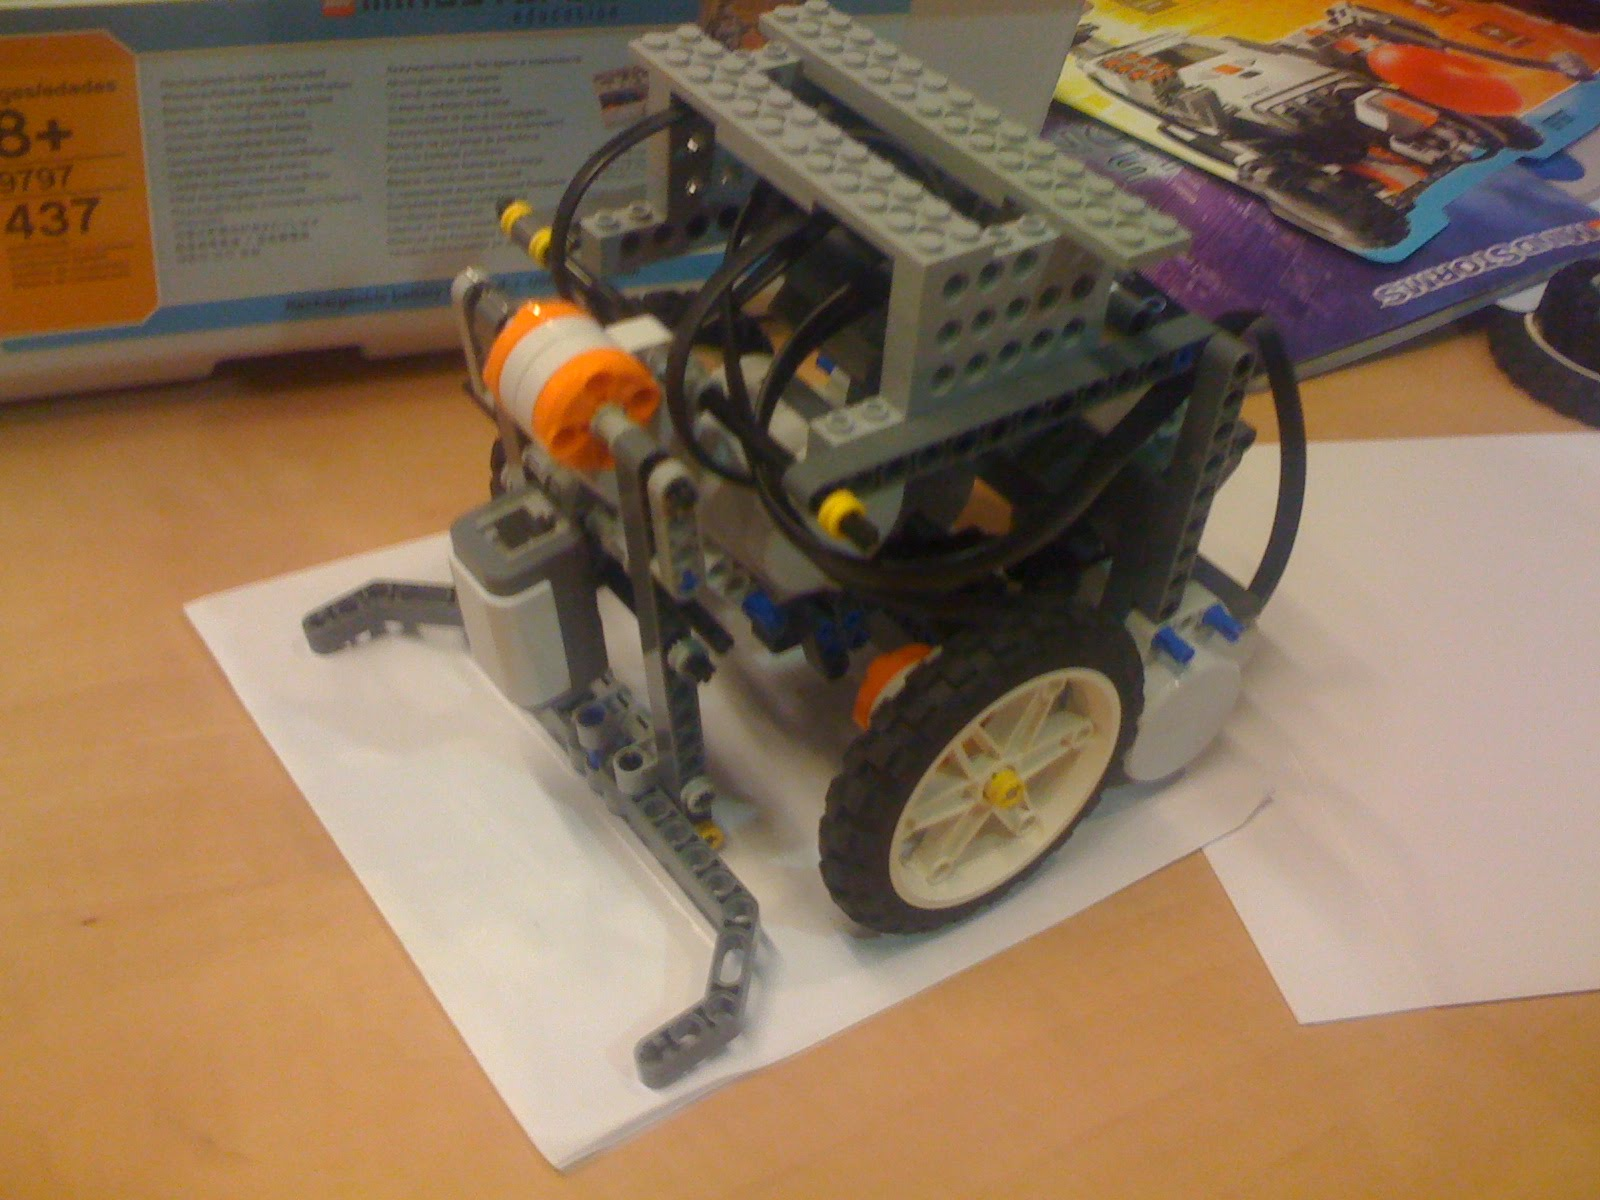
\includegraphics[width=0.4\textwidth] {robot2.png}
\end{center}
\caption{The robot design used in the first milestone demonstration}
\label{fig:robotDemo}
\end{figure}
\pagebreak

\begin{figure}[htp]
\begin{center}
\leavevmode
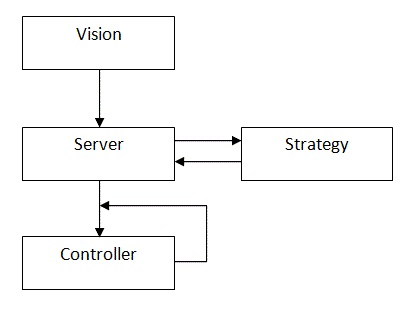
\includegraphics[width=0.4\textwidth] {diagram1.png}
\end{center}
\caption{Flow of data through the system}
\label{fig:dataFlow}
\end{figure}

\begin{figure}[htp]
\begin{center}
\leavevmode
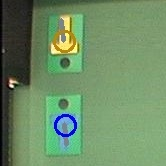
\includegraphics[width=0.4\textwidth] {vision2.jpg}
\end{center}
\caption{Object and orientation detection}
\label{fig:vision1}
\end{figure}

\begin{figure}[htp]
\begin{center}
\leavevmode
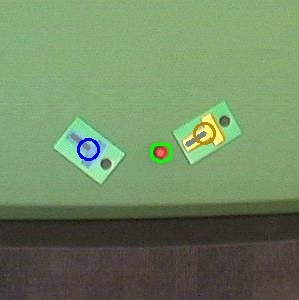
\includegraphics[width=0.3\textwidth] {vision3.jpg}
\end{center}
\caption{Robustness against shadows}
\label{fig:vision2}
\end{figure}

\begin{figure}[htp]
\begin{center}
\leavevmode
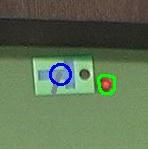
\includegraphics[width=0.3\textwidth] {vision1.jpg}
\end{center}
\caption{Inaccurate result for robot orientation}
\label{fig:vision3}
\end{figure}

\end{document}
